\begin{figure}
    \centering
    \begin{tikzpicture}
        \node[inner sep=0pt] (profile) at (0,0)
    {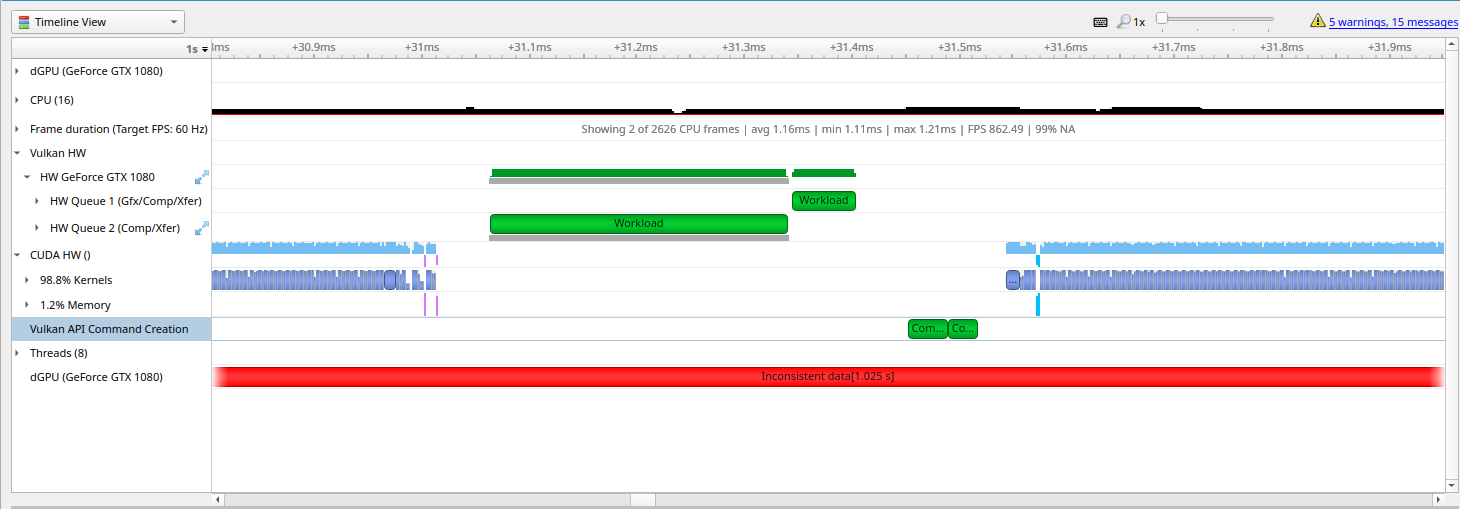
\includegraphics[width=1.0\linewidth]{Ch62Results/figures/temp_viz_profile.png}};
        
    \draw[line width=0.5mm,-Triangle] (-3.7, -0.5) -- ++(0, 1.8) -- ++(-0.21,0.0);% node[anchor=north east,align=right,fill=white] {GPU Reductions};
    % \draw[ultra thick,black,-Triangle] (vc.south west) -- (sim.north east) |- ++(0.25,0.5) ;
    \draw[line width=0.5mm] (-2.8, -0.5) -- ++(0,2);
    % \draw[line width=0.1mm] (-3.7, 1) -- (-2.8, 1);

    \draw[line width=0.5mm,-Triangle] (1.5, -0.5) -- ++(0, 1.8) -- ++(-0.21,0.0);
    \draw[line width=0.5mm] (3.2, -0.5) -- ++(0,2);
    
    % \draw[line width=0.1mm] (0.2, 1) -- (0.9, 1);
    
    \node[fill=white] at (-3.25, 1.8) {\SI{70}{\micro\second}};
    \node[fill=white] at (2.35, 1.8) {\SI{140}{\micro\second}};
    \end{tikzpicture}    
    \caption{Visualization Profile, highlighting the GPU bubbles}
    \label{fig:results:viz_profile_bubble}
\end{figure}
% the visualization work itself waits for around \SI{70}{\micro\second} before starting
%\todomark{This is time from semaphore, not time from reduction end, mark that on the graph}).
